\documentclass[12pt]{article}
\usepackage[utf8]{inputenc}
\usepackage[T1]{fontenc}
\usepackage[polish]{babel}
\usepackage{lmodern}

\usepackage{graphicx}

\title{\vspace{-1.5in}Sprawozdanie - kNN}
\author{Sebastian Michoń 136770, Marcin Zatorski 136834\\ grupa L5, czwartek 08:00}
\date{}

\begin{document}

\maketitle

\section{Wstęp}
Celem zadania było przetestowanie klasyfikatora kNN na zbiorze z danymi o jakości czerwonych win. Zbiór zawiera 11 atrybutów i około 1600 przykładów, klasa decyzyjna to jakość wina, jej możliwe wartości to: poor, medium i good.

\section{Zadanie}

Zbiór podzielono na treningowy (80\% przykładów) i testowy (20\% przykładów). Podział został wykonany przy użyciu metody \texttt{train\_test\_split} w scikit-learn, z domyślnymi parametrami, a więc został zastosowany shuffle, ale nie stratyfikacja.

Do przeskalowania danych użyto standaryzacji (StandardScaler). Każdy atrybut został przeskalowany niezależnie od siebie i zgodnie z wzorem:

\begin{equation}
z = \frac{x - \mu}{\sigma}
\end{equation}
\begin{enumerate}
	\item[$\mu$] - Średnia wartość atrybutu
	\item[$\sigma$] - Odchylenie standardowe wartości atrybutu
\end{enumerate}
Średnią i odchylenie standardowe obliczano tylko na zbiorze treningowym (także podczas walidacji krzyżowej, a więc nie uwzględniano wtedy zbioru walidacyjnego).

\begin{figure}[htb!]
	\centering
	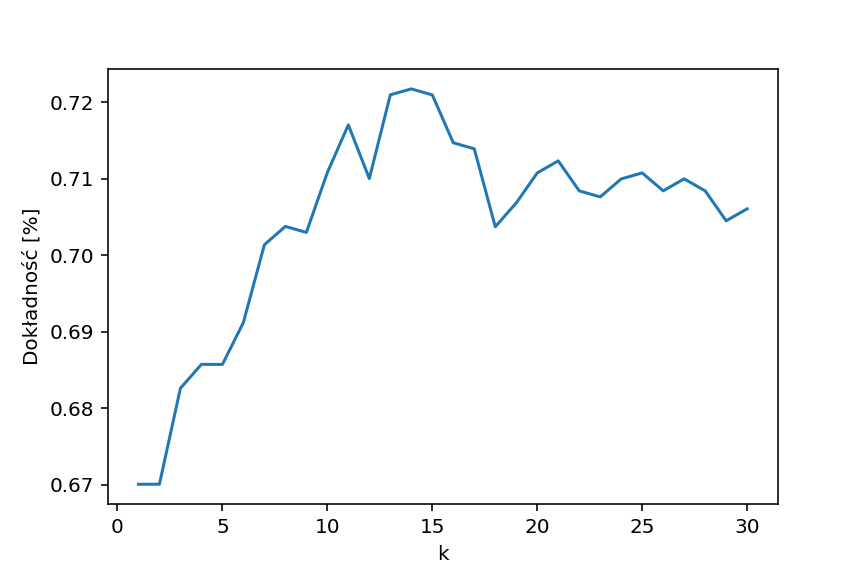
\includegraphics[width=0.7\columnwidth]{accuracy_knn.png}
	\caption{Dokładności w zależności od k}
	\label{fig:accuracy}
\end{figure}

Do klasyfikacji użyto klasyfikatora k najbliższych sąsiadów. Do obliczenia klasy użyto wag - waga sąsiada była odwrotnością odległości do niego. Taka waga osiągała wyższą dokładność - około 70\% w porównaniu do 60\% przy przypisywaniu sąsiadom równej wagi.

Klasyfikator przetestowano dla k od 1 do 30, używając walidacji krzyżowej ze stratyfikacją (domyślne ustawienie), z 10 podziałami. Wyniki dla każdego k uśredniono i przedstawiono na wykresie \ref{fig:accuracy}. Wyniki rosną od 67\% dla $k=1$ do 72\% dla k od 13 do 15, a następnie spadają do około 70\% dla wyższych k. Najwyższą dokładność uzyskano dla k równego 14 - a więc takie wybrano. Na zbiorze testowym dla $k=14$ klasyfikator uzyskał dokładność 70\%.

Przeprowadzono też testy różnych rodzajów skalowania - StandardScaler, MinMaxScaler i MaxAbsScaler. Wyniki i dokładność w zależności od k zamieszczono na wykresie \ref{fig:accuracy-scalers}. Najlepiej wypadł StandardScaler, następnie MinMaxScaler, a najgorzej MaxAbsScaler. Dla małych wartości k wyniki są porównywalne i szybko rosną, stabilizując się od k równego około 20.

\begin{figure}[htb!]
	\centering
	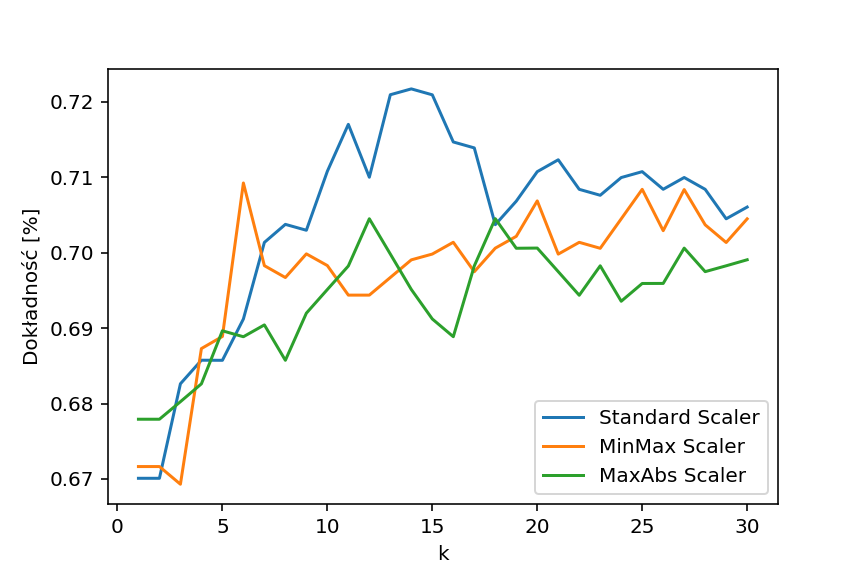
\includegraphics[width=0.7\columnwidth]{accuracy_scalers.png}
	\caption{Dokładność w zależności od k dla różnych rodzajów skalowania}
	\label{fig:accuracy-scalers}
\end{figure}

\end{document}
